\documentclass{beamer}
\setbeamertemplate{navigation symbols}{}
%% Black and white: the default theme colours structure and bibliography entries blue.
\setbeamercolor{structure}{fg=black}
\setbeamercolor{bibliography entry author}{fg=black}
\setbeamercolor{bibliography entry note}{fg=black}
\setbeamertemplate{bibliography item}{\insertbiblabel}

\usepackage[utf8]{inputenc}
\usepackage{amssymb}
\usepackage{tikz}
\usetikzlibrary{arrows.meta,positioning,shapes.geometric}
%% The one accent colour: marks what is formalized in CSLib (dark blue, dark grey in print).
\definecolor{cslib}{RGB}{0,63,135}

%% Notation, copied from ../papers/tcs/preamble.tex (without its amsthm setup, which clashes
%% with beamer's theorem environments).
\newcommand{\Atoms}{\mathbb{A}}
\newcommand{\Lam}{\Lambda}
\newcommand{\LamA}{\Lambda_{\alpha}}
\newcommand{\LamDB}{\mathrm{dB}}
\newcommand{\alphaeq}{=_{\alpha}}
\newcommand{\cls}[1]{[#1]_{\alpha}}
\newcommand{\lam}[2]{\lambda #1.\,#2}
\newcommand{\occ}{\mathrm{occ}}
\newcommand{\free}{\mathrm{free}}
\newcommand{\nocc}{\mathrel{\ntriangleright}}
\newcommand{\fresh}{\mathrel{\#}}
\newcommand{\sw}[2]{(#1\;#2)}
\newcommand{\act}{\cdot}
\newcommand{\subst}[3]{#1[#2 \mathrel{{:}{=}} #3]}
\newcommand{\simp}{\sim_{\mathrm{p}}}
\newcommand{\simpf}{\sim_{\mathrm{p}\#}}
\newcommand{\simpi}[1]{\sim^{#1}_{\mathrm{p}}}
\newcommand{\simr}{\sim_{\mathrm{r}}}
\newcommand{\simrf}{\sim_{\mathrm{r}\#}}
\newcommand{\infrule}[3]{\dfrac{#2}{#3}\;\textsc{#1}}
\newcommand{\dV}{\mathsf{dV}}
\newcommand{\dAPP}{\mathsf{dAPP}}
\newcommand{\dABS}{\mathsf{dABS}}
\newcommand{\dLAM}{\mathsf{dLAM}}
\newcommand{\lift}{\mathsf{lift}}
\newcommand{\nsub}{\mathsf{nsub}}
\newcommand{\dbsub}{\mathsf{sub}}
\newcommand{\tod}{\to_{\mathrm{d}}}
\newcommand{\todp}{\to_{\mathrm{d}'}}
\newcommand{\tobeta}{\to_{\beta}}
\newcommand{\tobetastar}{\twoheadrightarrow_{\beta}}
\newcommand{\supp}{\mathrm{supp}}
\newcommand{\inc}{\mathsf{inc}}
\newcommand{\ren}[3]{#1\langle #2 \mapsto #3\rangle}

%% Lean links, as in the paper. The paper's \leanicon looks for figures/lean-logo.pdf relative
%% to the current directory, so it is redefined to point at the paper's copy of the logo.
% Usage: \lean{https://github.com/leanprover/cslib/blob/<sha>/<path>.lean\#L<line>}
% typesets a small raised Lean logo that links to the declaration, attached to the preceding word.
% Put the official logo at figures/lean-logo.pdf; without it a plain turnstile is used.
\usepackage{graphicx}
\newcommand{\leanicon}{%
  \IfFileExists{figures/lean-logo.pdf}%
    {\includegraphics[height=0.85ex]{figures/lean-logo.pdf}}%
    {\ensuremath{\scriptstyle\vdash}}}
\newcommand{\lean}[1]{\ifhmode\unskip\fi\kern0.15em\href{#1}{\raisebox{0.9ex}{\leanicon}}}

\renewcommand{\leanicon}{%
  \IfFileExists{../papers/tcs/figures/lean-logo.pdf}%
    {
\includegraphics[height=0.85ex]{../papers/tcs/figures/lean-logo.pdf}}%
    {\ensuremath{\scriptstyle\vdash}}}
\newcommand{\LeanRepo}{https://github.com/chris-anto-froeschl/cslib}
\newcommand{\LeanPath}{Cslib/Languages/LambdaCalculus}
%% Crole, Theorem 4.1 and its prerequisites: the PR branch alpha-equivalence-equalities (#741).
\newcommand{\PRRev}{b69754c2fd59c7b9310439553495261524d1643d}
%% Crole, everything else: branch alpha-equivalence-equalities-rest (same pin as the paper).
\newcommand{\CroleRev}{d1883216c714d69b88282de195ab9e9250b23a05}
%% Norrish and Vestergaard: branch debruijn-alpha-quotient, pinned to the pushed head.
\newcommand{\DBRev}{8bdc761d35eb25e254d577a05da8b818e3af5d7d}
%% Number of the CSLib pull request with the de Bruijn isomorphism, as in the paper.
%% TODO: set it once the pull request is open.
\newcommand{\DBPR}{TODO}
\newcommand{\PRSrc}{\LeanRepo/blob/\PRRev/\LeanPath}
\newcommand{\CroleSrc}{\LeanRepo/blob/\CroleRev/\LeanPath}
\newcommand{\DBSrc}{\LeanRepo/blob/\DBRev/\LeanPath}
%% The worked example (CSLib's test file), pinned to the pushed head that contains it.
\newcommand{\DemoSrc}{\LeanRepo/blob/aaba16d7d4186b9947b2b7c1b35720260d253604/CslibTests/LambdaCalculus.lean}
%% TODO: re-pin the three revisions before the talk if the branches move.

\title{A Formalized Foundation for Research in Untyped Lambda Calculus}
\subtitle{Alpha equivalence and de Bruijn terms in Lean~4}
\author{Chris Anto Fr\"oschl}
\institute{Munich University of Applied Sciences}
\date{}

\begin{document}

\begin{frame}
  \titlepage
\end{frame}

%% ---------------------------------------------------------------- motivation

\begin{frame}{Context}
  \begin{itemize}
    \item Crole~\cite{crole2012a}: five textbook definitions of $\alphaeq$ define the same
      relation (widely accepted; published proof sketches are sometimes wrong).
    \item Norrish and Vestergaard~\cite{norrish2007a}: named terms modulo $\alphaeq$ and pure
      de Bruijn terms are isomorphic as reduction systems (mechanized in HOL4).
    \item Both formalized in Lean~4 on CSLib's two untyped $\lambda$-calculi:
      named terms with $\alphaeq$ (\#458~\cite{cslib458}) and de Bruijn terms with $\beta$
      and Church--Rosser (\#475, open~\cite{cslib475}).
    \item Status: Crole's Theorem~4.1 in review (\#741~\cite{cslib741}), the isomorphism in
      review (\#\DBPR); Crole's other theorems on a branch; no \texttt{sorry} in what is
      presented here.
    \item Blueprint with a dependency graph of both formalizations and their connections:
      \href{https://chris-anto-froeschl.github.io/untyped-lambda-calculus/}{\footnotesize\texttt{chris-anto-froeschl.github.io/untyped-lambda-calculus}}
    \item Today: how the proofs go, in particular the parts we have not discussed yet.
  \end{itemize}
\end{frame}

%% ---------------------------------------------------------------- Crole

\begin{frame}{Live: a worked example in CSLib}
  An example file that uses the formalization, stepped through in the editor
  (\texttt{CslibTests/LambdaCalculus.lean} \lean{\DemoSrc\#L64}). Every step is checked by
  Lean.
  \begin{enumerate}
    \item[(a)] The three operations on $M = \lam{a}{a\,b}$: renaming, swap, substitution.
    \item[(b)] The five relations on $\lam{a}{a\,b}$ and $\lam{c}{c\,b}$, from $\alphaeq$ through
      Crole's theorems and directly by each relation's own rule.
    \item[(c)] The counterexamples of Proposition~4.3.
    \item[(d)] De Bruijn: $f$ on the running example, the bijection, one $\beta$-step on both
      sides (Theorem~20), Church--Rosser for $\LamA$.
  \end{enumerate}
\end{frame}

\begin{frame}{Operations on atoms}
  \small
  \begin{itemize}
    \item Renaming $\ren{M}{a}{b}$
      \lean{\PRSrc/Named/Untyped/Basic.lean\#L70}:
      every occurrence of $a$ (free, bound or binding) replaced by $b$. Purely textual.
    \item Permutation action $\pi \act M$
      \lean{\PRSrc/Named/Untyped/AlphaEquivVariants/Defs.lean\#L71}:
      a bijection $\pi$ on atoms applied to every atom, binders included:
      \[ \pi \act a = \pi(a) \quad \pi \act (M_1\,M_2) = (\pi \act M_1)\,(\pi \act M_2)
         \quad \pi \act \lam{a}{M} = \lam{\pi(a)}{\pi \act M} \]
      The \emph{swap} $\sw{a}{b} \act M$
      \lean{\PRSrc/Named/Untyped/AlphaEquivVariants/Defs.lean\#L82}
      is the case of a transposition.
    \item Capture-avoiding substitution $\subst{M}{a}{N}$
      \lean{\PRSrc/Named/Untyped/Basic.lean\#L116}:
      replaces the free occurrences of $a$ by $N$, and renames a binder to a fresh atom
      when it would capture a free atom of $N$ (Curry style).
  \end{itemize}
  For $M = \lam{a}{a\,b}$:
  \begin{align*}
    \ren{M}{a}{b} &= \lam{b}{b\,b} && \text{identifies $a$, $b$; captures the free $b$}\\
    \sw{a}{b} \act M &= \lam{b}{b\,a} && \text{exchanges $a$ and $b$}\\
    \subst{M}{b}{a} &= \lam{c}{c\,a} && \text{only the free $b$; binder renamed, $c$ fresh}
  \end{align*}
\end{frame}

\begin{frame}{Five alpha equivalences \cite[Defs.~3.1--3.5]{crole2012a}}
  Swapping relations: congruence for atoms and applications, plus
  \[
    \infrule{pi}{\sw{z}{a} \act M \sim \sw{z}{b} \act M'}{\lam{a}{M} \sim \lam{b}{M'}}
  \]
  \begin{center}
  \begin{tabular}{lll}
    $\simp$ & $z \nocc a, b, M, M'$ & CSLib's $\alphaeq$
      \lean{\PRSrc/Named/Untyped/Basic.lean\#L82}\\
    $\simpf$ & $z \fresh a, b, M, M'$ & \lean{\PRSrc/Named/Untyped/AlphaEquivVariants/Defs.lean\#L89}\\
    $\simpi{1}$ & $z \nocc M, M'$ & \lean{\PRSrc/Named/Untyped/AlphaEquivVariants/Defs.lean\#L107}
  \end{tabular}
  \end{center}
  Renaming relations: equivalence, congruence, plus
  \[
    \infrule{$\alpha$}{}{\lam{a}{M} \sim \lam{a'}{\subst{M}{a}{a'}}}
  \]
  \begin{center}
  \begin{tabular}{lll}
    $\simr$ & $a' \nocc a, M$ & Barendregt
      \lean{\PRSrc/Named/Untyped/AlphaEquivVariants/Defs.lean\#L122}\\
    $\simrf$ & $a' \fresh a, M$ & Hindley--Seldin
      \lean{\PRSrc/Named/Untyped/AlphaEquivVariants/Defs.lean\#L142}
  \end{tabular}
  \end{center}
  {\footnotesize $a \nocc M$: $a$ does not occur in $M$ at all.
  $a \fresh M$: $a$ is not free in $M$.}
\end{frame}

\begin{frame}{Crole's theorem}
  \begin{theorem}[\cite{crole2012a}, Thms.~4.1, 4.2, 4.4--4.6]
    ${\simp} = {\simpf} = {\simpi{1}} = {\simr} = {\simrf}$.
  \end{theorem}
  \begin{center}
  \begin{tabular}{llll}
    4.1 & ${\simp} = {\simpf}$ & \lean{\PRSrc/Named/Untyped/AlphaEquivVariants/Equalities.lean\#L94}
      & in CSLib PR \#741\\
    4.2 & ${\simp} = {\simpi{1}}$ & \lean{\CroleSrc/Named/Untyped/AlphaEquivEquiv.lean\#L151}
      & follow-up branch\\
    4.4 & ${\simp} = {\simr}$ & \lean{\CroleSrc/Named/Untyped/AlphaEquivEquiv.lean\#L261}
      & follow-up branch\\
    4.5 & ${\simp} = {\simrf}$ & \lean{\CroleSrc/Named/Untyped/AlphaEquivEquiv.lean\#L324}
      & follow-up branch\\
    4.6 & ${\simr} = {\simrf}$ & & via 4.4 and 4.5
  \end{tabular}
  \end{center}
  \bigskip
  The side condition cannot be weakened much further
  (Prop.~4.3 \lean{\CroleSrc/Named/Untyped/AlphaEquivEquiv.lean\#L157}):
  \begin{itemize}
    \item only $z \nocc a, b$: \quad $\lam{a}{a\,z} \sim \lam{b}{b\,a}$
    \item no condition: \quad $\lam{a}{b\,a} \sim \lam{b}{a\,b}$
  \end{itemize}
  In both cases the free atoms differ, so the terms are not $\alphaeq$.
\end{frame}

\begin{frame}{Why swap and not substitute?}
  \begin{itemize}
    \item Renaming and substitution can identify two atoms:
      $\subst{(a\,b)}{a}{b} = b\,b$.
    \item A swap is a bijection on terms: it never identifies atoms, so it never captures,
      and it commutes with every operation that mentions no particular atom.
    \item With an unused atom swap and renaming agree: $z \nocc M$ implies
      $\sw{z}{a} \act M = \ren{M}{a}{z}$
      \lean{\PRSrc/Named/Untyped/AlphaEquivVariants/Swap.lean\#L138}.
      CSLib's $\alphaeq$ writes \textsc{pi} with this one-way renaming; under
      $z \nocc M$ it is Crole's rule. $\simpf$ must keep the swap: with only $z \fresh M$
      the two differ.
  \end{itemize}
\end{frame}

\begin{frame}{Two lemmas on permutations \cite[Lemmas~6.1, 6.2]{crole2012a}}
  \begin{block}{Lemma 6.1 \lean{\PRSrc/Named/Untyped/AlphaEquivVariants/Swap.lean\#L285}}
    $M \simp M'$ implies $\sw{u}{v} \act M \simp \sw{u}{v} \act M'$.
  \end{block}
  \begin{itemize}
    \item $\simp$ is equivariant. Rule induction; the \textsc{pi} case splits on how the atoms
      of the rule relate to $u$ and $v$: 27 cases, of which the paper shows representative
      ones. Lean: five helper lemmas for the representative cases and an explicit case tree
      covering all 27.
  \end{itemize}
  \begin{block}{Lemma 6.2}
    Let $\pi, \pi'$ agree on a set of atoms.
    \begin{enumerate}
      \item on $\occ(M)$: \ $\pi \act M = \pi' \act M$
        \lean{\PRSrc/Named/Untyped/AlphaEquivVariants/Swap.lean\#L91}
      \item on $\free(M)$: \ $\pi \act M \simp \pi' \act M$
        \lean{\PRSrc/Named/Untyped/AlphaEquivVariants/Swap.lean\#L379}
    \end{enumerate}
  \end{block}
  \begin{itemize}
    \item Part 2 says: up to $\alpha$, only the free atoms of a term matter (a support
      statement, see the nominal slides later). Lean: ``agree on $S$'' is Mathlib's
      \texttt{Set.EqOn $\pi$ $\pi'$ S}, for arbitrary bijections (Crole: finite support).
  \end{itemize}
\end{frame}

\begin{frame}{Proof of Theorem 4.1: ${\simp} = {\simpf}$}
  Lean: \texttt{alphaEquiv\_iff\_alphaEquivPFresh}
  \lean{\PRSrc/Named/Untyped/AlphaEquivVariants/Equalities.lean\#L94}.
  Each relation is closed under the rules of the other; only \textsc{pi} needs work.
  \begin{itemize}
    \item ${\simp} \subseteq {\simpf}$: $z \nocc M$ implies $z \fresh M$, so \textsc{pi} is an
      instance of \textsc{pi\#}.
    \item ${\simpf} \subseteq {\simp}$: given $\sw{u}{a} \act M \simp \sw{u}{b} \act M'$ with
      only $u \fresh a, b, M, M'$. Choose $z \nocc u, a, b, M, M'$.
      \begin{enumerate}
        \item Lemma~6.1 with $\sw{z}{u}$:
          $\sw{z}{u}\sw{u}{a} \act M \simp \sw{z}{u}\sw{u}{b} \act M'$.
        \item $\sw{z}{u} \circ \sw{u}{a}$ and $\sw{z}{a}$ agree on $\free(M)$, since
          $u, z \notin \free(M)$. Lemma~6.2(2):
          $\sw{z}{u}\sw{u}{a} \act M \simp \sw{z}{a} \act M$
          \lean{\PRSrc/Named/Untyped/AlphaEquivVariants/Swap.lean\#L413}.
        \item Same on the right; symmetry and transitivity give
          $\sw{z}{a} \act M \simp \sw{z}{b} \act M'$, the premise of \textsc{pi}.
      \end{enumerate}
    \item Symmetry and transitivity of $\simp$ come from \#458, proved directly. Crole gets
      them later, from Theorem~4.4: the Lean dependency order differs from the paper's.
  \end{itemize}
\end{frame}

\begin{frame}{The renaming relations: Theorems 4.4 and 4.5}
  Bridge: swapping with an unused atom is, up to $\simr$, substitution
  \cite[Lemmas~6.3, 6.4]{crole2012a}:
  \[
    z \nocc M \implies \sw{z}{a} \act M \simr \subst{M}{a}{z}
    \lean{\CroleSrc/Named/Untyped/AlphaEquivLemmas.lean\#L167}
    \quad (\text{and } \simrf
    \lean{\CroleSrc/Named/Untyped/AlphaEquivLemmas.lean\#L203})
  \]
  \begin{itemize}
    \item \textsc{pi} $\Rightarrow$ $\simr$: \
      $\lam{a}{M} \simr \lam{z}{\subst{M}{a}{z}} \simr \lam{z}{\subst{M'}{b}{z}}
      \simr \lam{b}{M'}$ \ by $\alpha$, \textsc{bcg}, $\alpha$.
    \item $\alpha$ $\Rightarrow$ $\simp$: for $a' \fresh M$ and fresh $z$,
      $\sw{z}{a} \act M \simp \sw{z}{a'} \act \subst{M}{a}{a'}$ \
      (Lemma~6.5, $n = 1$ \lean{\CroleSrc/Named/Untyped/AlphaEquivLemmas.lean\#L476}).
  \end{itemize}
  \begin{block}{Departure}
    Crole proves the $\alpha$ case by induction on $M$, which fails for $\alpha\#$
    ($\subst{M}{a}{a'}$ may rename a binder), and repairs it with Lemma~6.5 for $n$ swaps.
    We prove only $n = 1$, with $z \fresh M$ where Crole assumes $z \nocc M$: one lemma
    serves both $\simr$ and $\simrf$.
  \end{block}
\end{frame}

\begin{frame}{What the formalization had to add to \cite{crole2012a}}
  \begin{itemize}
    \item Existence of substitution (deferred in the paper): Gabbay's definition~\cite[Def.~5.13]{gabbay2011a};
      well defined by induction on size~\cite[L.~5.14]{gabbay2011a}.
    \item Lemma~6.1: all 27 cases, not representatives.
    \item Lemma~6.2(1): omitted in the paper.
    \item Lemmas~6.5 and~6.6: details omitted or ``well known''.
    \item A small change of hypotheses (Lemma~6.5, previous slide). No errors found in the
      paper.
  \end{itemize}
\end{frame}

\begin{frame}{Where Crole's Section 6.1 lemmas come from}
  \small
  Crole names a source only for 6.3; the others are what we found.
  \medskip

  \begin{tabular}{@{}lll@{}}
    Lemma & Proof in~\cite{crole2012a} & Earlier source \\
    \hline
    6.1 & representative cases & \cite[pf.~of Prop.~2.2]{gabbay2002a}, \cite[(9)]{urban2004a} \\
    6.2(1) & omitted & \cite[Ex.~3.5(ii)]{gabbay2002a} \\
    6.2(2) & given & \cite[L.~2.8]{urban2004a}, \cite[L.~3.8]{gabbay2008a} \\
    6.3, 6.4 & given & \cite[L.~5.16]{gabbay2011a}, \cite[L.~3.6(2)]{gabbay2008a} \\
    6.5 & details omitted & $n{=}1$: \cite[pf.~of Prop.~2.2]{gabbay2002a} + \cite[A1.7--8]{hindley2008a} \\
    6.6 & ``well known'' & \cite[L.~A1.5(g)]{hindley2008a} \\
  \end{tabular}
  \medskip

  \begin{itemize}
    \item Gabbay and Pitts call 6.1 and the $\simp$-form of 6.3 ``easily verified'' when
      proving that $\simp$ is $\alpha$; Crole (p.~5) notes their sketch also needs 6.3 for
      $\simr$.
    \item 6.5 for general $n$: our own induction; Crole's earlier Hybrid paper has no swapping.
  \end{itemize}
\end{frame}

%% ---------------------------------------------------------------- Norrish and Vestergaard

\begin{frame}{The claim \cite{norrish2007a}}
  Two reduction systems:
  \begin{itemize}
    \item $\langle \LamA, \tobeta \rangle$: named terms modulo $\alphaeq$, ordinary $\beta$
      \lean{\DBSrc/Named/Untyped/AlphaQuotient.lean\#L115}
    \item $\langle \LamDB, \tod \rangle$: pure de Bruijn terms, Nipkow's $\beta$
      \lean{\DBSrc/Unscoped/Untyped/BetaReduction.lean\#L41}
  \end{itemize}
  \begin{block}{Theorem 20}
    There is a bijection $f \colon \LamA \to \LamDB$ with
    \[ M \tobeta N \iff f(M) \tod f(N). \]
  \end{block}
  \begin{itemize}
    \item Why ``$\iff$''? For relations a bijective homomorphism is not enough:
      the identity $\langle \mathbb{N}, \emptyset \rangle \to \langle \mathbb{N}, < \rangle$
      preserves the relation but is no isomorphism.
    \item Both relations: one contraction rule plus congruence rules
      (left, right, under a binder).
  \end{itemize}
\end{frame}

%% Figure 1 of Norrish and Vestergaard, with the TikZ code of the paper's Figure
%% (../papers/tcs/sections/future-work.tex, label fig:equivalence-net); only the row labels are
%% broken onto two lines to fit the slide. Keep the two in sync.
%% TODO: extend for the talk (CSLib's current nodes and edges, planned ones).
\begin{frame}{Where the result sits}
  \begin{center}
  \resizebox{\linewidth}{!}{%
  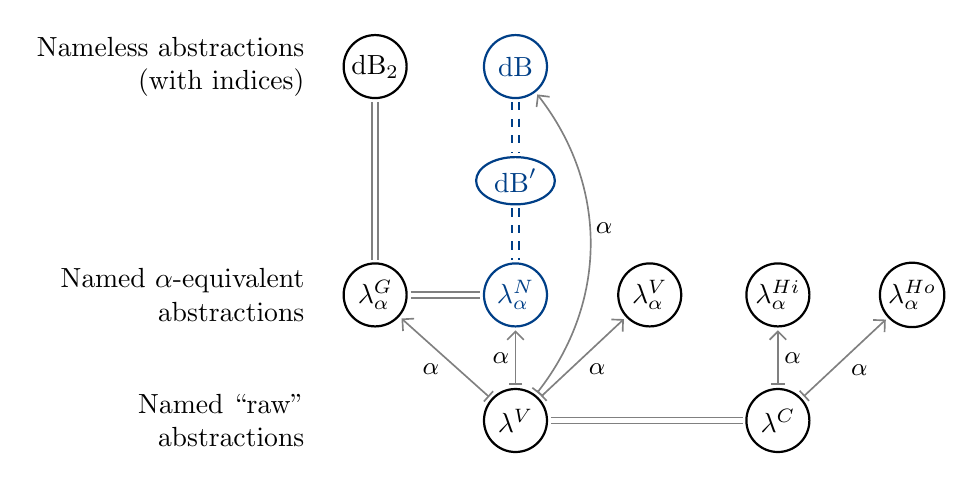
\begin{tikzpicture}[
      x=1.55cm, y=1.45cm,
      sys/.style={draw, thick, circle, inner sep=1pt, minimum size=8mm},
      iso/.style={semithick, double, double distance=1.5pt, draw=black!50, shorten <=1pt, shorten >=1pt},
      new/.style={double, double distance=1.5pt, thick, dashed, draw=cslib, shorten <=1pt, shorten >=1pt},
      cs/.style={draw=cslib, text=cslib},
      quo/.style={semithick, draw=black!50, {Bar[width=5pt]}-{Straight Barb[length=3pt]}, shorten <=1pt, shorten >=1pt},
      lab/.style={font=\small, inner sep=2pt}]
    \node[anchor=east, align=right] at (-0.5, 2) {Nameless abstractions\\(with indices)};
    \node[anchor=east, align=right] at (-0.5, 0) {Named $\alpha$-equivalent\\abstractions};
    \node[anchor=east, align=right] at (-0.5,-1.1) {Named ``raw''\\abstractions};

    \node[sys] (dB2) at (0, 2) {$\mathrm{dB}_2$};
    \node[sys, cs] (dB)  at (1.15, 2) {$\mathrm{dB}$};
    \node[sys, cs, ellipse, minimum size=0pt, minimum width=10mm, minimum height=6mm]
              (dBp) at (1.15, 1) {$\mathrm{dB}'$};
    \node[sys] (lG)  at (0, 0) {$\lambda^{G}_{\alpha}$};
    \node[sys, cs] (lN)  at (1.15, 0) {$\lambda^{N}_{\alpha}$};
    \node[sys] (lVa) at (2.25, 0) {$\lambda^{V}_{\alpha}$};
    \node[sys] (lHi) at (3.3, 0) {$\lambda^{Hi}_{\alpha}$};
    \node[sys] (lHo) at (4.4, 0) {$\lambda^{Ho}_{\alpha}$};
    \node[sys] (lV)  at (1.15,-1.1) {$\lambda^{V}$};
    \node[sys] (lC)  at (3.3,-1.1) {$\lambda^{C}$};

    \draw[iso] (dB2) -- (lG);
    \draw[iso] (lG) -- (lN);
    \draw[iso] (lV) -- (lC);
    \draw[new] (dB) -- (dBp);
    \draw[new] (dBp) -- (lN);

    \draw[quo] (lV) -- node[lab, below left] {$\alpha$} (lG);
    \draw[quo] (lV) -- node[lab, left] {$\alpha$} (lN);
    \draw[quo] (lV) -- node[lab, below right] {$\alpha$} (lVa);
    \draw[quo] (lV) to[bend right=38] node[lab, right, pos=0.55] {$\alpha$} (dB);
    \draw[quo] (lC) -- node[lab, right] {$\alpha$} (lHi);
    \draw[quo] (lC) -- node[lab, below right] {$\alpha$} (lHo);
  \end{tikzpicture}}
  \end{center}
  \medskip
  {\footnotesize Formalizations of the untyped $\lambda$-calculus and their directly proved
  relationships, redrawn from \cite[Figure~1]{norrish2007a}. Double lines are isomorphisms,
  arrows are $\alpha$-quotients. The dashed lines are the results of~\cite{norrish2007a},
  \textcolor{cslib}{formalized here in Lean}.\par}
  \medskip
  {\footnotesize Our $\LamA$ is the quotient by $\simp$, the relation HOL4 also uses for
  $\lambda^N_\alpha$; by Crole's theorem it is also the quotient by $\simr$ (Barendregt) and
  $\simrf$ (Hindley--Seldin). Substitution is lifted from raw terms, as in
  $\lambda^{Ho}_\alpha$.\par}
\end{frame}

\begin{frame}{Reading de Bruijn terms}
  \[ t \;::=\; \dV\, i \mid \dAPP\, t\, t \mid \dABS\, t \]
  \begin{itemize}
    \item A bound index counts the binders up to its own binder.
    \item A free index $i$ is the $i$-th name of a naming context
      $\Gamma = [a, b, c, \dots]$; every binder pushes its variable to the front.
  \end{itemize}
  \medskip
  Examples, with $\Gamma = [a, b, c, \dots]$:
  \begin{itemize}
    \item $\lam{f}{\lam{x}{f\,x}} = \dABS\,(\dABS\,(\dAPP\,(\dV\,1)\,(\dV\,0)))$
    \item applied to the free $\dV\,5$:
      \[ \tod \;\dABS\,(\dAPP\,(\dV\,6)\,(\dV\,0)) \]
      under the remaining binder, the free $5$ is now called $6$.
    \item $(\lam{x}{x\,a})\,b$ is $\dAPP\,(\dABS\,(\dAPP\,(\dV\,0)\,(\dV\,1)))\,(\dV\,1)$
      \[ \tod\; \dAPP\,(\dV\,1)\,(\dV\,0) \;=\; b\,a. \]
  \end{itemize}
\end{frame}

\begin{frame}{$\lift$ and $\nsub$ \cite{nipkow2001a}}
  \begin{itemize}
    \item $\lift\, t\, k$ adds $1$ to the free indices $\geq k$
      \lean{\DBSrc/NamedDeBruijn/PureDeBruijn.lean\#L68}:
      keeps them pointing at the right name under a new binder.
      \begin{itemize}
        \item $\lift\,(\dV\,3)\,0 = \dV\,4$, \quad $\lift\,(\dV\,3)\,5 = \dV\,3$
        \item $\lift\,(\dABS\,(\dAPP\,(\dV\,0)\,(\dV\,2)))\,0
          = \dABS\,(\dAPP\,(\dV\,0)\,(\dV\,3))$
          \hfill ($\lam{x}{x\,b}$: $x$ stays, $b$ moves)
      \end{itemize}
    \item $\nsub\, s\, k\, t$ substitutes $s$ for $k$ and closes the gap above $k$
      \lean{\DBSrc/NamedDeBruijn/PureDeBruijn.lean\#L81}:
      \begin{itemize}
        \item at $k = 1$: \ $\dV\,0 \mapsto \dV\,0$, \ $\dV\,1 \mapsto s$,
          \ $\dV\,2 \mapsto \dV\,1$
        \item $\nsub\,(\dV\,5)\,0\,(\dAPP\,(\dV\,0)\,(\dV\,3)) = \dAPP\,(\dV\,5)\,(\dV\,2)$
      \end{itemize}
    \item Both parts are needed:
      \begin{itemize}
        \item $(\lam{x}{x\,a})\,b$ without the decrement gives $b\,b$.
        \item $(\lam{x}{\lam{y}{x}})\,a$: \ $\nsub\,(\dV\,0)\,0\,(\dABS\,(\dV\,1))
          = \dABS\,(\dV\,1) = \lam{y}{a}$; without the $\lift$ inside $\nsub$ it would be
          $\dABS\,(\dV\,0) = \lam{y}{y}$.
      \end{itemize}
  \end{itemize}
\end{frame}

\begin{frame}{The route}
  \begin{center}
  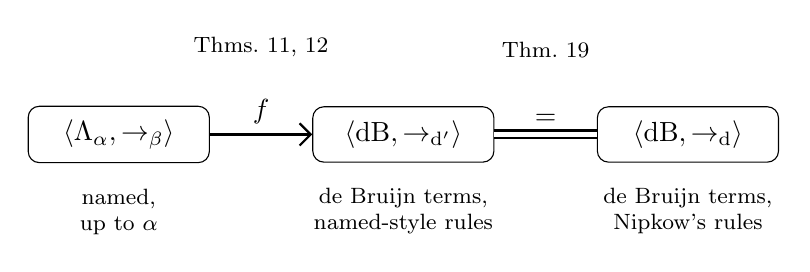
\begin{tikzpicture}[
      sys/.style={draw, rounded corners, inner sep=5pt, minimum width=2.3cm},
      lab/.style={font=\footnotesize, align=center},
      >={Straight Barb[length=4pt]}]
    \node[sys] (la) {$\langle \LamA, \tobeta \rangle$};
    \node[sys, right=1.3cm of la] (dbp) {$\langle \LamDB, \todp \rangle$};
    \node[sys, right=1.3cm of dbp] (db) {$\langle \LamDB, \tod \rangle$};
    \draw[->, thick] (la) -- node[above] {$f$} (dbp);
    \draw[double, thick, double distance=2pt] (dbp) -- node[above] {$=$} (db);
    \node[lab, above=0.5cm of la.north east, xshift=0.65cm] {Thms.~11, 12};
    \node[lab, above=0.5cm of dbp.north east, xshift=0.65cm] {Thm.~19};
    \node[lab, below=0.2cm of la] {named,\\ up to $\alpha$};
    \node[lab, below=0.2cm of dbp] {de Bruijn terms,\\ named-style rules};
    \node[lab, below=0.2cm of db] {de Bruijn terms,\\ Nipkow's rules};
  \end{tikzpicture}
  \end{center}
  \begin{itemize}
    \item $\LamDB'$: the same terms, but with a binder $\dLAM\, i$ over a chosen index and a
      substitution $\dbsub$ that leaves the other indices alone.
    \item Thm.~12: $f$ turns $\tobeta$ into $\todp$. Easy, because $\LamDB'$ is built to
      look like $\LamA$.
    \item Thm.~19: $\todp = \tod$. The hard part:
      contraction rules by Lemma~13, binder rules by Thm.~15.
  \end{itemize}
\end{frame}

\begin{frame}{$\LamDB'$: a named-style binder on de Bruijn terms}
  \begin{itemize}
    \item $\dbsub\, s\, k\, (\dV\, i) = \text{if } i = k \text{ then } s \text{ else } \dV\, i$
      \lean{\DBSrc/NamedDeBruijn/PureDeBruijn.lean\#L99}
      \hfill (no gap closing)
    \item $\dLAM\, i\, t = \dABS\, (\dbsub\, (\dV\, 0)\, (i + 1)\, (\lift\, t\, 0))$
      \lean{\DBSrc/NamedDeBruijn/PureDeBruijn.lean\#L217}
      \\ \hfill (bind the free $i$)
  \end{itemize}
  $\dLAM$ forgets which name it bound, like $\lambda$ on $\LamA$:
  \begin{itemize}
    \item $\dLAM\,0\,(\dV\,0) = \dLAM\,1\,(\dV\,1) = \dABS\,(\dV\,0)$
      \hfill ($\lam{a}{a}$, $\lam{b}{b}$)
    \item $\dLAM\,0\,(\dAPP\,(\dV\,0)\,(\dV\,1)) = \dLAM\,2\,(\dAPP\,(\dV\,2)\,(\dV\,1))$\\
      \hfill $= \dABS\,(\dAPP\,(\dV\,0)\,(\dV\,2))$
      \quad ($\lam{a}{a\,b}$, $\lam{c}{c\,b}$)
  \end{itemize}
  Every $\dABS$ term is a $\dLAM$ term over any index not free in it
  (Lemma~6 \lean{\DBSrc/NamedDeBruijn/PureDeBruijn.lean\#L280}).
  \medskip

  $\todp$ \lean{\DBSrc/NamedDeBruijn/PureDeBruijn.lean\#L369}:
  $\dAPP\,(\dLAM\, i\, t)\, u \todp \dbsub\, u\, i\, t$, and congruences with
  $\dLAM\, i$ in place of $\dABS$.
\end{frame}

\begin{frame}{Nominal ideas, by example (1)}
  Slogan: only the relationships between names matter, not the names themselves.
  \medskip

  Names $a, b, c, d$; permutations act on everything built from names:
  \begin{itemize}
    \item $\sw{a}{b} \act a = b$, \quad $\sw{a}{b} \act 5 = 5$,
      \quad $\sw{a}{b} \act \{a, c\} = \{b, c\}$, \quad $\sw{a}{b} \act \{a, b\} = \{a, b\}$
  \end{itemize}
  Support: the names a permutation has to fix to fix the object.
  \begin{center}
  \begin{tabular}{ll}
    object & support\\\hline
    $a$ & $\{a\}$\\
    $5$ & $\emptyset$\\
    $\{a, c\}$ & $\{a, c\}$\\
    raw term $\lam{a}{a\,b}$ & $\{a, b\}$ \quad all its names, $\occ$\\
    class $\cls{\lam{a}{a\,b}}$ & $\{b\}$ \quad free names only, $\free$
  \end{tabular}
  \end{center}
  $\sw{a}{c}$ keeps the class ($\lam{c}{c\,b} \alphaeq \lam{a}{a\,b}$), $\sw{b}{c}$ does
  not. Quotienting by $\alpha$ turns ``all names'' into ``free names''
  (Crole's Lemma~6.2, parts 1 and 2).
\end{frame}

\begin{frame}{Nominal ideas, by example (2)}
  Equivariant: commutes with every permutation, i.e.\ mentions no particular name.
  \begin{itemize}
    \item Equivariant: $\free$, size, $\alphaeq$, $\tobeta$.
      \\ E.g.\ $\lam{a}{a} \alphaeq \lam{b}{b}$, and after $\sw{a}{c}$:
      $\lam{c}{c} \alphaeq \lam{b}{b}$.
    \item Not equivariant: ``$a \in \free(M)$'' (true for $a$, false for $b$).
    \item Not equivariant: $\mathrm{fresh}(S)$ = the smallest name not in $S$:
      \\ $\mathrm{fresh}\{a\} = b$, but $\mathrm{fresh}\{c\} = a \neq \sw{a}{c} \act b$.
  \end{itemize}
  \medskip
  Consequences for the paper:
  \begin{itemize}
    \item A function out of $\LamA$ may only use names equivariantly.
      $f \colon \LamA \to \LamDB$ is fine; a direct $\LamDB \to \LamA$ would have to
      invent names.
    \item Permutations act on de Bruijn terms through the free indices
      (Def.~8 \lean{\DBSrc/NamedDeBruijn/DeBruijnPerm.lean\#L169});
      $\dbsub$, $\dLAM$ and $\todp$ are equivariant
      (Thm.~10 \lean{\DBSrc/NamedDeBruijn/DeBruijnPerm.lean\#L336}).
  \end{itemize}
\end{frame}

\begin{frame}{The bijection $f$ (Thms.~11, 12)}
  \begin{gather*}
    f(\cls{a}) = \dV\, \hat{a}
    \qquad
    f(M\, N) = \dAPP\, (f\, M)\, (f\, N)
    \\
    f(\lam{a}{M}) = \dLAM\, \hat{a}\, (f\, M)
  \end{gather*}
  {\footnotesize $\hat{a}$: the number of the atom $a$.}
  \begin{itemize}
    \item The paper: Pitts' recursion principle for $\LamA$, which needs $\LamDB$ as a
      nominal set.
    \item Lean: structural recursion on raw terms
      \lean{\DBSrc/NamedDeBruijn/FromTerm.lean\#L113},
      shown to respect $\alphaeq$
      \lean{\DBSrc/NamedDeBruijn/FromTerm.lean\#L203},
      then lifted to the quotient
      \lean{\DBSrc/NamedDeBruijn/FromTerm.lean\#L390}.
      Possible because $\dLAM$ forgets the name.
    \item Injective: $\dLAM$ is injective up to a swap
      \lean{\DBSrc/NamedDeBruijn/LiftingPermutation.lean\#L332}.
      Surjective: by size, using Lemma~6.
    \item Substitution: $f(\subst{M}{a}{N}) = \dbsub\, (f\, N)\, \hat{a}\, (f\, M)$
      \lean{\DBSrc/NamedDeBruijn/FromTerm.lean\#L256}
    \item Thm.~12: $M \tobeta N \iff f(M) \todp f(N)$
      \lean{\DBSrc/NamedDeBruijn/FromTerm.lean\#L476}
  \end{itemize}
\end{frame}

\begin{frame}{The key observation: $\lift$ is a permutation}
  \begin{block}{Lemma 14 \lean{\DBSrc/NamedDeBruijn/LiftingPermutation.lean\#L144}}
    If all free indices of $t$ are $\leq n$, then $\lift\, t\, m = \pi_{m,n} \act t$
    for the cycle $\pi_{m,n} \colon m \mapsto m{+}1 \mapsto \dots \mapsto n{+}1 \mapsto m$.
  \end{block}
  Example: $\lift\,(\dAPP\,(\dV\,0)\,(\dV\,2))\,0 = \dAPP\,(\dV\,1)\,(\dV\,3)$ is the cycle
  $0 \to 1 \to 2 \to 3 \to 0$; index $3$ is unused in $t$, so it can wrap around.
  \medskip
  \begin{block}{Theorem 15 \lean{\DBSrc/NamedDeBruijn/LiftingPermutation.lean\#L358}}
    For an equivariant $R$: \ $R$ is closed under $\dABS$ $\iff$
    $R$ is closed under every $\dLAM\, i$.
  \end{block}
  \begin{itemize}
    \item $\dABS\,t$ and its presentation as a $\dLAM$ term differ by a permutation, and an
      equivariant relation cannot see permutations.
    \item Lemma~13 \lean{\DBSrc/NamedDeBruijn/LiftingPermutation.lean\#L54} matches the
      contraction rules:
      $\dbsub\, u\, i\, t = \nsub\, u\, n\, (\dbsub\, (\dV\, n)\, (i{+}1)\, (\lift\, t\, n))$
      for $n \leq i$.
  \end{itemize}
\end{frame}

\begin{frame}{Equivariance of $\tod$: Lemma 17}
  Theorem~15 needs $\tod$ to be equivariant. $\todp$ is (Theorem~10), but $\tod$ is built
  from $\nsub$, which does not commute with permutations in the obvious way.
  \begin{itemize}
    \item Naive: permute everything. With $\pi = \sw{0}{1}$:
      \begin{align*}
        \pi \act \nsub\,(\dV\,5)\,0\,(\dV\,1) &= \pi \act \dV\,0 = \dV\,1\\
        \nsub\,(\pi \act \dV\,5)\,0\,(\pi \act \dV\,1) &= \nsub\,(\dV\,5)\,0\,(\dV\,0) = \dV\,5
      \end{align*}
  \end{itemize}
  \begin{block}{Lemma 17 \lean{\DBSrc/NamedDeBruijn/Isomorphism.lean\#L61}}
    $\pi \act (\nsub\, t\, i\, u) = \nsub\, (\pi \act t)\, i\, (\inc_i(\pi) \act u)$
  \end{block}
  \begin{itemize}
    \item The index $i$ is not permuted, and the body gets the incremented permutation:
      $\inc_0\sw{0}{1} = \sw{1}{2}$, so $\nsub\,(\dV\,5)\,0\,(\dV\,2) = \dV\,1$. Correct.
    \item Reason: $\nsub$ at $i$ removes a binder, so the body lives one level deeper.
    \item With it, $\tod$ is equivariant by rule induction, and Lemma~18 follows from
      Theorem~15.
  \end{itemize}
\end{frame}

\begin{frame}{Theorems 19 and 20 in Lean}
  \begin{itemize}
    \item Thm.~19: $t \todp u \iff t \tod u$
      \lean{\DBSrc/NamedDeBruijn/Isomorphism.lean\#L126}
    \item Thm.~20 = Thm.~12 + Thm.~19
      \lean{\DBSrc/NamedDeBruijn/Isomorphism.lean\#L146}
  \end{itemize}
  \medskip
  As a Mathlib relation isomorphism
  \lean{\DBSrc/NamedDeBruijn/Isomorphism.lean\#L151}:
  \begin{block}{}
    \small
    \texttt{noncomputable def dbRelIso :}\\
    \quad\texttt{BetaAlpha (Var := Atom)} $\simeq_r$ \texttt{Beta :=}\\
    \quad$\langle$\texttt{dbEquiv, betaAlpha\_iff\_beta.symm}$\rangle$
  \end{block}
  \begin{itemize}
    \item $r \simeq_r s$: an equivalence $e$ with $s\,(e\,a)\,(e\,b) \iff r\,a\,b$,
      exactly the paper's notion of isomorphic systems.
    \item No \texttt{sorry}; Thm.~20 depends only on \texttt{propext},
      \texttt{Classical.choice}, \texttt{Quot.sound}.
    \item $f^{-1}$ comes from surjectivity by choice, so it is not computable.
  \end{itemize}
\end{frame}

\begin{frame}{Payoff: Church--Rosser for free}
  \begin{itemize}
    \item \#475 proves Church--Rosser for $\tod$
      \lean{\DBSrc/Unscoped/Untyped/ChurchRosser.lean\#L45}.
    \item An isomorphism of reduction systems transports everything stated in terms of
      the relation: $\twoheadrightarrow$, confluence, normal forms.
  \end{itemize}
  \begin{block}{Corollary}
    $\tobeta$ on $\LamA$ is confluent
    \lean{\DBSrc/NamedDeBruijn/Transfer.lean\#L147}:
    if $M \tobetastar N_1$ and $M \tobetastar N_2$, there is $P$ with
    $N_1 \tobetastar P$ and $N_2 \tobetastar P$.
  \end{block}
  \begin{block}{Corollary}
    $\beta$-normal forms on $\LamA$ are unique
    \lean{\DBSrc/NamedDeBruijn/Transfer.lean\#L220}.
  \end{block}
  \begin{itemize}
    \item No further work on the named side; not in~\cite{norrish2007a}.
  \end{itemize}
\end{frame}

\begin{frame}{Departures from the papers}
  \begin{itemize}
    \item Crole's \textsc{pi} is stated with renaming instead of a swap; equal under its
      side condition.
    \item $\alphaeq$ is reflexive, symmetric, transitive by direct proofs (from \#458), not
      via Theorem~4.4.
    \item $\LamA$ substitution is lifted from raw terms, and so is $f$; no Pitts recursion.
    \item Atoms: natural numbers in a wrapper, where the paper has strings with a bijection
      to $\mathbb{N}$.
    \item Permutations are finitely supported bijections, not lists of pairs.
    \item $\lift$, $\nsub$, $\dbsub$ are \#475's operations; the paper's equations are lemmas.
    \item No general notion of equivariant relation: Thm.~15 takes equivariance as a
      hypothesis.
  \end{itemize}
\end{frame}

\begin{frame}{Status and future work}
  \begin{itemize}
    \item Crole: follow-up PRs after \#741 (Thms.~4.2, 4.4--4.6, Prop.~4.3).
    \item Norrish and Vestergaard: in review (\#\DBPR), on top of \#475 and \#741.
      % TODO: size of the de Bruijn files (2,310 lines, 135 theorems on 2026-10-13)?
    \item The $\eta$ version of Thm.~20 is also proved
      \lean{\DBSrc/NamedDeBruijn/Eta.lean\#L302}.
      % TODO: keep or drop eta, as in the paper.
    \item Next:
      \begin{itemize}
        \item more representations (locally nameless, nominal), connected by explicit
          isomorphisms;
        \item Crole-style equivalences elsewhere, e.g.\ SK combinators;
        \item the remaining nodes and edges of Figure~1 of~\cite{norrish2007a}
          (slide ``Where the result sits''): $\mathrm{dB}_2$, $\lambda^V$, $\lambda^C$ and
          their $\alpha$-quotients;
        \item teaching: Fabrizio Montesi (University of Southern Denmark) and Alexandre
          Rademaker (Getulio Vargas Foundation), both CSLib maintainers, are interested in
          using the named representation for lectures and assignments on the
          $\lambda$-calculus.
      \end{itemize}
  \end{itemize}
\end{frame}

\begin{frame}[allowframebreaks]{References}
  \nocite{cslib,cslib458,cslib475,cslib741}
  \scriptsize
  \bibliographystyle{plain}
  \bibliography{../papers/tcs/refs,colloquium}
\end{frame}

\end{document}
